\chapter{Analysis}\label{analysis}

\section{Introduction}\label{analysis:intro}
The creation of an embedded system presents many issues as it interacts with a physical environment which can throw many different exceptions. Embedded systems must be able to handle these exceptions to maintain its integrity.

Henzinger and Sifakis claim they’re two key areas of constraints on embedded systems in physical environments, reaction constraints and execution constraints. Reaction constraints include deadlines, bandwidth capable on the data buses and jitter. The execution constraints refer to processing speeds and power that the system must be able to handle/ keep up with. [1]

When thinking about the different constraints I would have to work within for my project these two areas certainly formed a basis on which I built my requirements and choose my relevant hardware.

In terms of the reaction constraints, deadlines will be highly important and will certainly affect how I schedule my tasks and manage shared resources. I will be giving the task which posts the recorded data to the mobile application very strict and precise deadlines so that the task responsible for monitoring the boards movements is given as much time on the CPU as possible when the system is running. Jitter could be overcome through implementing a time triggered system but this kind of system also presents problems such as high latency which I can avoid by using an event triggered architecture. This is something that I must consider and is discussed in more depth in this literature review.

In terms of execution constraints, I do not have any problems, the microcontroller I have chosen to use is an Arduino 101 this board has a clock speed of 32 MHz [2] which will be more than enough processing power to perform the tasks that are needed by my system to collect data from sensors and send this data to a mobile application via Bluetooth. 

The power that system needs to be able to handle won’t be a problem either as the power supply for the board will need to small enough so that it fits on the skateboard without effecting the ability to use a great deal. This influenced the decision to choose a 9V power supply for my board which is perfect as the recommend voltage supply for this board is between 7 – 12 V with the board operating at 3.3V [2].

\section{Embedded Systems Issues}\label{analysis:embeddedsystems}
\subsection{System Reliability}\label{analysis:esreliability}
Reliability and Efficiency is going to be a key aspect in this project and I must consider the systems reliability it two mains areas, collecting the data from the sensors correctly and then sending it to the phone reliably. In a way, I am subject to a catch 22 type of situation where increased reliability may mean the efficiency of the system decreases and vice versa. For example, if I look at how I am going to develop the embedded system for this project I could weigh up critical systems engineering against best-effort engineering. These are two very different approaches; critical systems engineering is best suited for hard real time systems where as best effort is favoured for soft embedded systems.

“The hard-real time approach leads to low utilisation of system resources. On the other hand, soft approaches take the risk of temporary unavailability” [1] Applying this to the system I want to create I would opt for a best effort soft real time system approach as I will be utilising several system resources such as the accelerometer, gyroscope, Bluetooth chip and possibly pressure sensors. I will be using some if not all (at times) of these resources is tandem so going for a hard time approach such as critical systems engineering may be costly to how efficiently the system will run.

By choosing a soft real time approach I will have more dynamic resource allocation which will be important when using several different components on my microcontroller at the same time. This will also allow me to consider other performance metrics such system performance to be taken equally as seriously. [3]

The down side to this however is I may experience degradation of the systems integrity; I could run into issues where tasks of some data capturing components experience starvation and are blocked of their ability to be able to post their data onto the data bus. This issue could be avoided using hard real time approach as I could schedule the system to give each component and task a set block of time using the processor to post the data. This however I can still overcome this in soft real-time system by implementing buffers to store the data into until the bus becomes available. 

\subsection{Concurrency}\label{analysis:esconcurrency}
Concurrency is another problem within the embedded systems design challenge that I had to consider as parallelisation of processing tasks in digital signal processing tasks and algorithms is highly important and increases the systems capability. [4] 

I need a highly concurrent system as I will have at least 2 components capturing and posting data at the same time. Thus, I am planning on using a higher sample rate for the components such as the accelerometer and gyroscope than I initially planned. By doing this, if one components task is not able to run as the CPU is busy then less samples will be missed and the general pattern that performing the skate trick creates will be less distorted. 

I was initially going to set the sample rate at 80 samples per second (1 sample every 12.5 milliseconds) however if I scale this up and choose a sample rate of 160 samples per second I end up with 1 sample every 6.25 milliseconds. By doing this if a process if denied access to the CPU for 10 milliseconds it will miss 1 sample the same as using a sample rate of 80 however I will have twice the number of samples before and after to use to predict what the pattern would have looked like if the sample wasn’t missed.

Getting my systems concurrency correct is highly important to the project as a lot of tasks, critical to the overall system performance, will be running at the same time. For example, I will have tasks running that monitor the accelerometer and gyroscope at the same time alongside tasks responsible for processing the data and sending it off to the mobile application to be pushed up to internet. The way that I will do this is by following a model coined by Norbert Schramm which can be seen in the figure below [4]: 
\begin{figure}[h]
\begin{center}
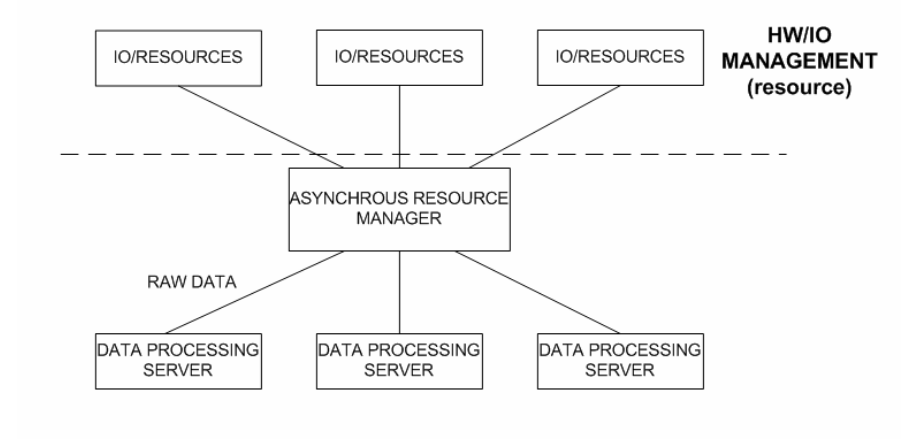
\includegraphics[width=.75\textwidth]{ANALYSIS/fig1.png}
\end{center}
\caption{Asynchronous Resource Manager}
\end{figure}

As you can see they’re several I/O resources that feed into an asynchronous resource manager which provides access for the data processing elements. In terms of my project the IO/Resources boxes on the diagram represent my accelerometer, gyroscope and pressure sensors as these are the components providing the raw data. 

The asynchronous resource manager block you see in the middle will be the Bluetooth data protocol that allows the mobile application access to the data, it was also oversee what order messages are getting sent in. The mobile phone in the case of the diagram is the data processing server. The reason that mobile phone takes the role of the data processing server is that according Schramm’s explanation of the model the role of the data processing server is to convert raw data (which is what will be given by the accelerometer during run time into a specific data type which provides input for an action to be executed. 

This now gives me all the components needed for an execution module. Using the method presented by Schramm the execution module is just simply a lightweight thread, here is an example of a thread [4]:
\begin{figure}[h]
\begin{center}
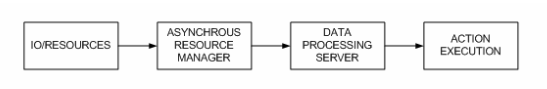
\includegraphics[width=.75\textwidth]{ANALYSIS/fig2.png}
\end{center}
\caption{Execution cycle for a general thread}
\end{figure}

Having a light weight thread means that I reduce my resource requirements and gain faster context switching which is something that I require for my system to operate the best it can. Fast context switching is desired in my system as I want post data as quickly as possible so that the tasks responsible for capturing the data have as much time on the CPU as possible so that the data readings are as accurate as they can be.

\subsection{Time Triggered vs Event Triggered}\label{analysis:esttvset}
Running a concurrent system will lead me onto my next consideration which is the style of interrupts I should use in the system for the microcontroller. For this I have two options; time triggered interrupts or event triggered interrupts. Time- triggered (TT) systems are best suited for regular operation of distributed control systems but with them include the issue of high latency across the systems various buses, however time triggered architectures remove any possible jitter between tasks. [5] This is something that would be highly desirable to my system as I want system to be very efficient during context switching so that when the task to post recorded data to the phone runs the CPU is given back to tasks responsible for recording the data as quick as possible. 

On the other hand, with time triggered events carrying the burden of high latency I feel that this will cancel out the fact this architecture removes jitter from the equation. If there is a high latency on the data bus the tasks which post the data to the mobile phone may have to spend time on the CPU waiting for the data to arrive from the tasks monitoring the various sensors around the board. 

In addition to this the very way I want my system to work is event triggered, if there is a sudden change in the values of any of the sensors then this must mean a trick has been performed at this point I will want to make sure that the tasks responsible for posting the data and sending it to the phone can run. In an event triggered system data is sent immediately using an interrupt mechanism whereas with time triggered systems there can be a delay based on the polling period of the TT system. [6] This reinforces my decision to develop an event triggered system, I will be able to send data off the mobile as soon as a trick is performed using a ISR and I will also reduce the latency within my software.

\section{Sourcing the Hardware}\label{anaylsis:sourcinghardware}

\subsection{Bluetooth Low Energy}\label{anaylsis:bluetoothLE}

Roughly 60\% of packets were succesfully transmitted over BLE

https://www.eecs.umich.edu/courses/eecs589/papers/06215496.pdf

\section{Neural Networks}\label{anaylsis:neuralnetwork}

\subsection{Rule Based Nueral Networks}\label{anaylsis:ruledbasedNN}




